Similar to the previous section, we will first describe the metric system researchers used to evaluate the models that do 3D pose estimation, and then we will demonstrate the results and the comparisons. The Dataset that we are going to use for this evaluation is the Human3.6M dataset \cite{Human3.6M}. The Human3.6M dataset is one of the largest motion capture datasets, which consists of 3.6 million human poses and corresponding images captured by a high-speed motion capture system. There are 4 high-resolution progressive scan cameras to acquire video data at 50 Hz. The dataset contains activities by 11 professional actors in 17 scenarios: discussion, smoking, taking photo, talking on the phone, etc., as well as provides accurate 3D joint positions and high-resolution videos. We employ a variation of the standard mean per joint position error (MPJPE) metric to evaluate our models. The MPJPE metric is the root-relative Euclidean error averaged over all joints and poses. In a root-relative pose, the hip (the root joint) is set at the origin. Since we are interested in coordinates in a global space, we do not move the hip to the origin. We call the latter metric Absolute MPJPE or A-MPJPE for short. The original MPJPE is called Relative or R-MPJPE to avoid confusion.\\

In absolute pose estimation there could be two sources of errors: the (root-relative) pose is incorrectly estimated, or the absolute location of the pose is incorrect. The scale of the second type of error can be much larger then the first type. We report both metrics to avoid that the absolute error hides an inaccurate pose prediction\\

To summarize, the definition of the metrics:

\begin{itemize}
  \item \textbf{A-MPJPE or Absolute MPJPE: }  The average Euclidean distance between the ground truth and  predicted joints in millimeters.
  \item \textbf{R-MPJPE or Relative MPJPE: } The average Euclidean distance between the ground truth and predicted hip-relative joint coordinates in millimeters. Previous work calls this the MPJPE metric.
\end{itemize} 
Thus, the A-MPJPE metric is a natural extension of the common MPJPE metric. The formula of the MPJPE for a frame f and a Skeleton S is: 

$$ E_{MPJPE}(f,S) = \dfrac{1}{N_S}\sum^{N_S}_{i=1} \lVert  m_{f,S}^{f}(i) - m_{gt,S}^{f}(i)   \rVert_2 $$
where, $N_S$ is the number of the joints in skeleton S. For a set of frames the error is the average over the MPJPEs of the frames.

\begin{figure}[h]
	\centering
	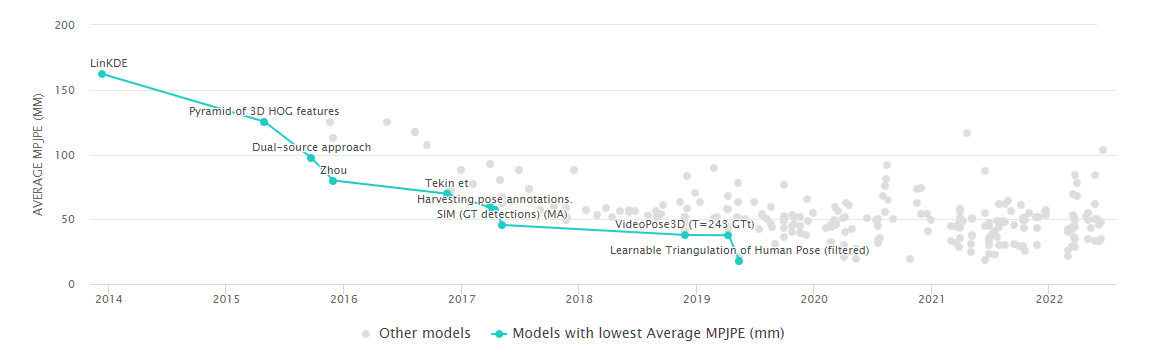
\includegraphics[width=1\textwidth]{figures/Evaluation/VideoPose3Dcomparison.png}
	\captionsetup{labelformat=empty}
	\caption{\href{https://paperswithcode.com/sota/3d-human-pose-estimation-on-human36m}
	{VideoPose3D model Average MPJPE tests evaluation compared to other keypoint Detection Models on Human3.6M Dataset.}}
\end{figure}

\pagebreak

\begin{figure}[h]
	\centering
	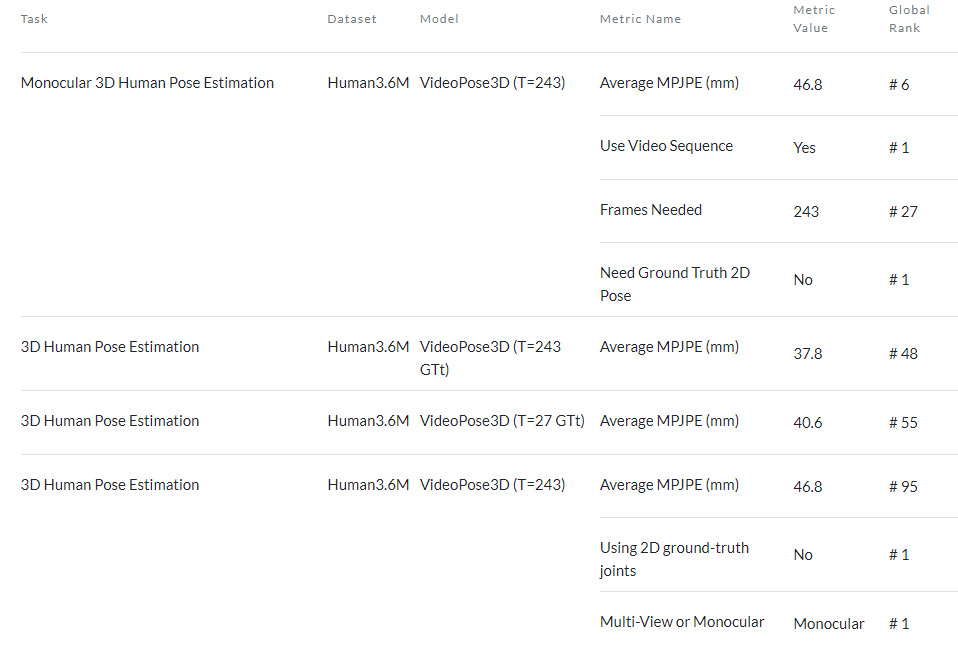
\includegraphics[width=0.8\textwidth]{figures/Evaluation/EvaluationVideoPose3D1.png}
	\captionsetup{labelformat=empty}
	\caption{\href{https://paperswithcode.com/paper/3d-human-pose-estimation-in-video-with}
	{VideoPose3D model Average MPJPE tests evaluation on Human3.6M Dataset}}
\end{figure}

\begin{figure}[h]
	\centering
	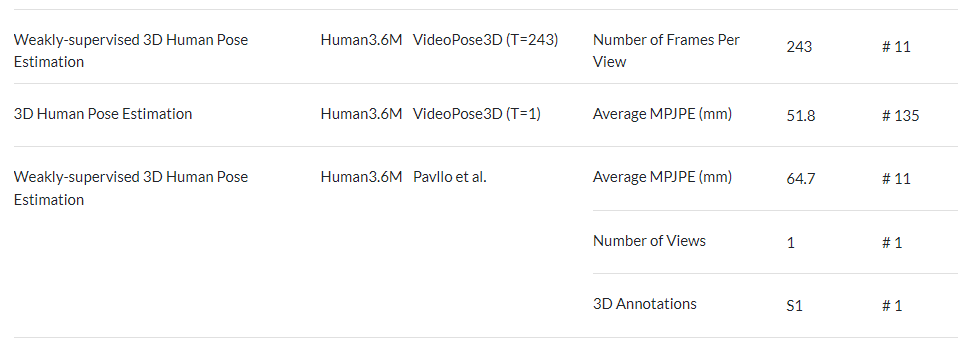
\includegraphics[width=0.8\textwidth]{figures/Evaluation/EvaluationVideoPose3D2.png}
	\captionsetup{labelformat=empty}
	\caption{\href{https://paperswithcode.com/paper/3d-human-pose-estimation-in-video-with}
	{VideoPose3D model Average MPJPE tests evaluation on Human3.6M Dataset}}
\end{figure}